\documentclass{beamer}
\usetheme{Madrid}

\usepackage{caption}
\usepackage{booktabs}
\usepackage{varwidth}
\usepackage{animate}

\usepackage{amsmath}

\usepackage{ragged2e}
\usepackage[style=ieee]{biblatex}
\setbeamertemplate{bibliography item}{\insertbiblabel}
\addbibresource{references.bib}

\title{Spoken Keyword Spotting}
\author{Vineeth S}
\centering
\date{July 2020}

\begin{document}
\justifying

\nocite{*}

\maketitle

\begin{frame}{Project Overview}
	\begin{itemize}
		\item<1-> Spoken Keyword Spotting is the task of identifying predefined words (called as keywords) from speech. 
		\item<2-> For the of this project, we will be using the Google Speech Commands Dataset\cite{gsc}.
		\item<3-> Speech Commands dataset has 65,000 one-second long utterances of 30 short words recorded by people with different demographics.
		\item<4-> For this project we will be using a single word as a keyword. The dataset also contains two names --- Marvin and Sheila --- out of which we use \textbf{Marvin }as our hotword (keyword).
	\end{itemize}
\end{frame}



\begin{frame}{KWS System Pipeline}
	\begin{itemize}
		\item<1-> The input to the system is via Tensorflow Dataset Object which provides efficient handling of large sized data, generating features in an ad-hoc fashion.
		\item<2-> The input feature for the system is the log Mel Filterbank energies of the speech signal calculated with a window of length $25ms$ and stepsize $10ms$.
		\item<3-> The keyword detection system comprises of two models --- a feature (embedding) extractor and a SVM classifier.
		\item<4-> The output of the system would be a binary value predicting whether the given speech sequence is a keyword.
	\end{itemize}
\end{frame}


\begin{frame}{Speech Commands Classifier}
	\begin{figure}[h]
		\centering
		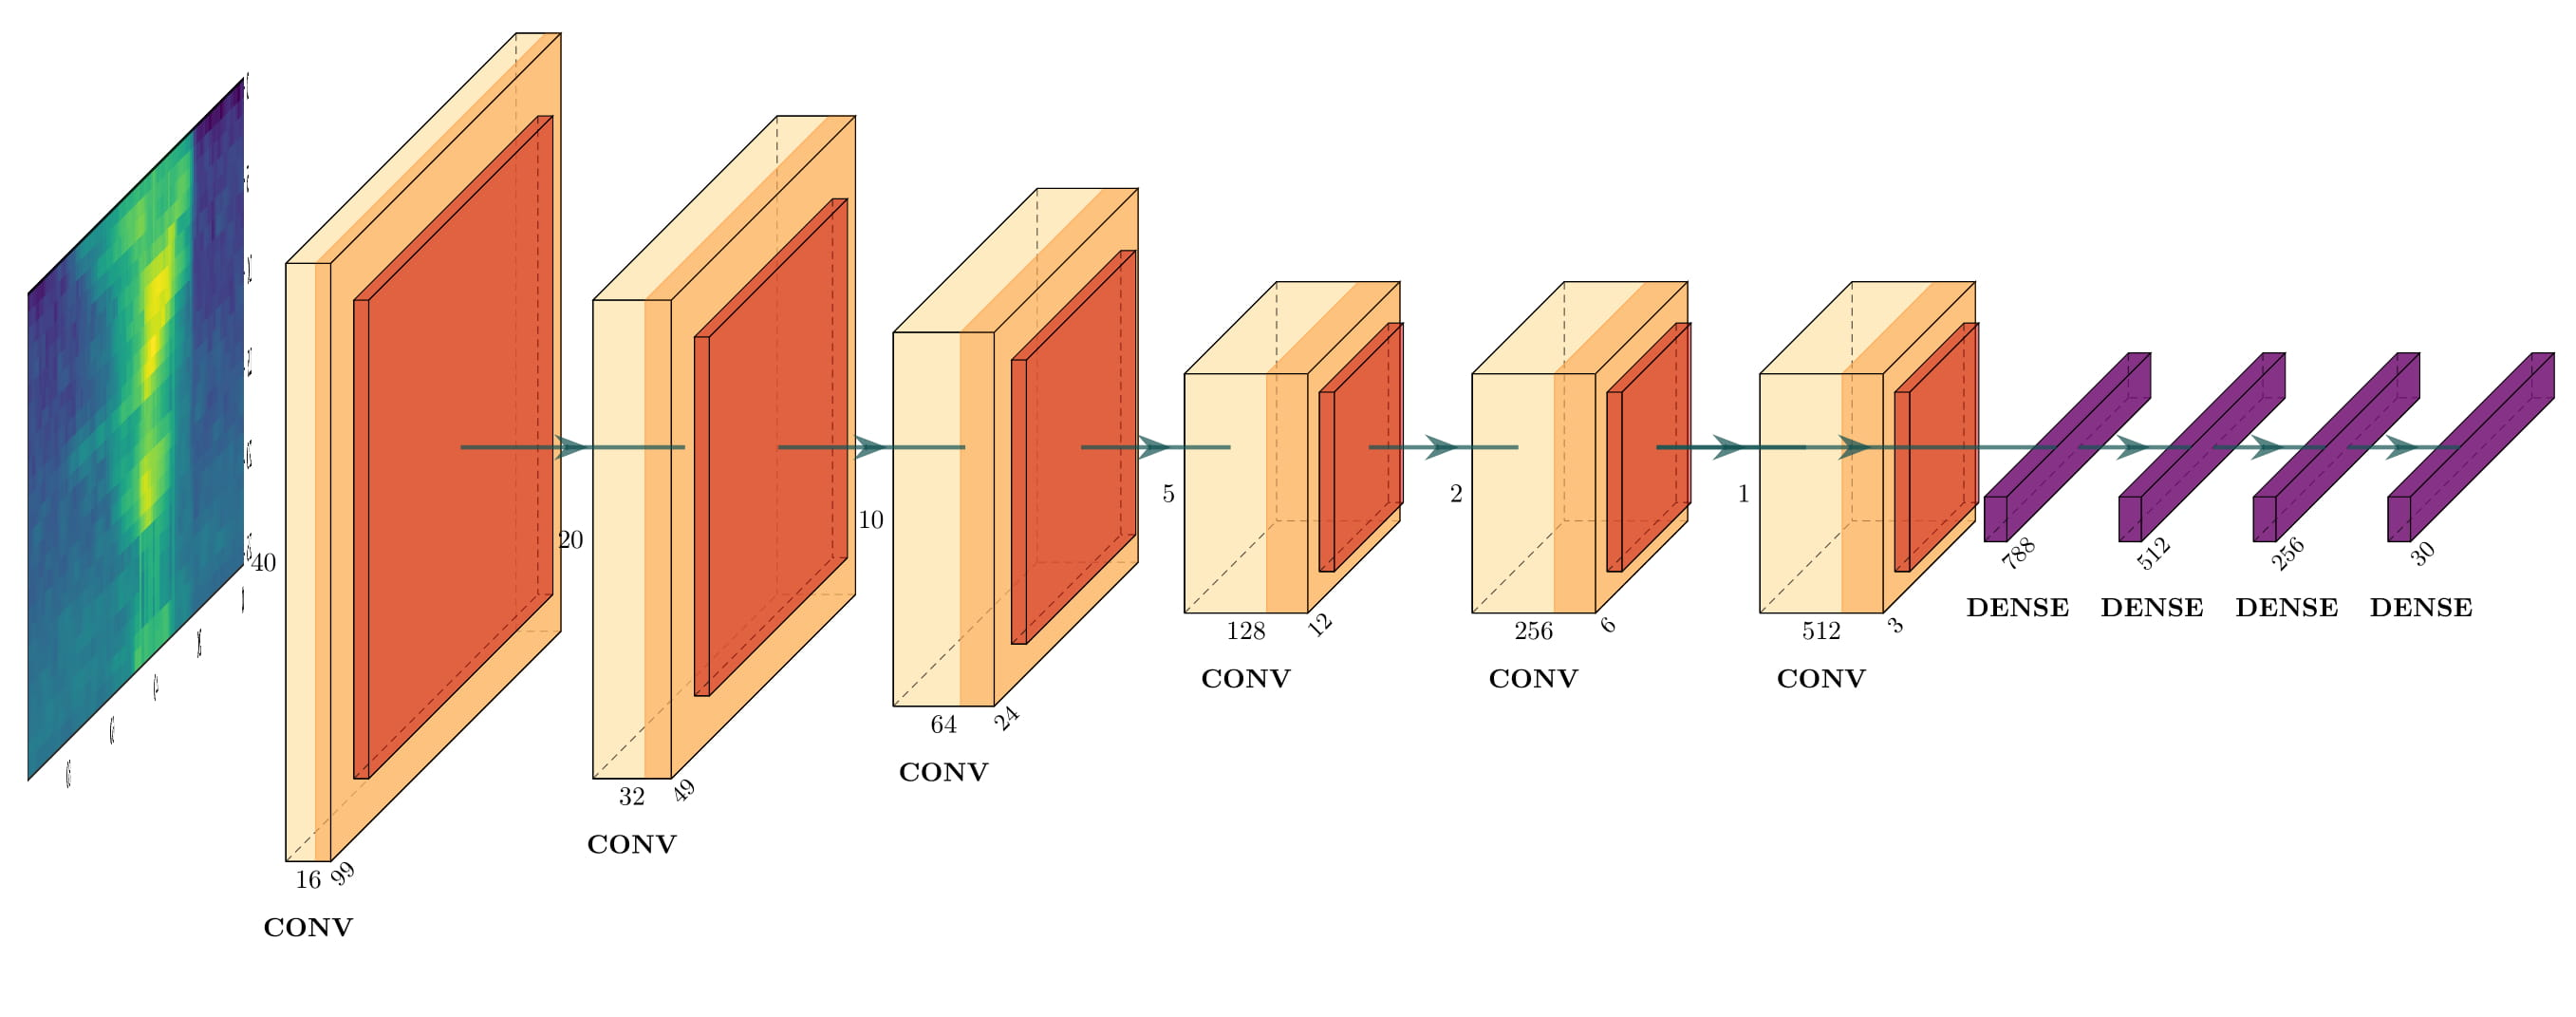
\includegraphics[width=1\linewidth, height=0.35\linewidth]{../results/kws1.jpg}
		%\caption{Word Classifier}
		\label{fig:feature}
	\end{figure}
	
	\begin{itemize}
   		\item<1-> The above is a word classifier for Speech Commands dataset. 
		\item<2-> This model achieves an training accuracy of 96.59\% and validation accuracy of 95.56\%.
		\item<3-> We are having a deep CNN architecture with $\sim$ 1000k parameters and sample processing time of $\sim$ 1.75ms.
	\end{itemize}
\end{frame}


\begin{frame}{Feature Extractor}
	\begin{figure}[h]
		\centering
		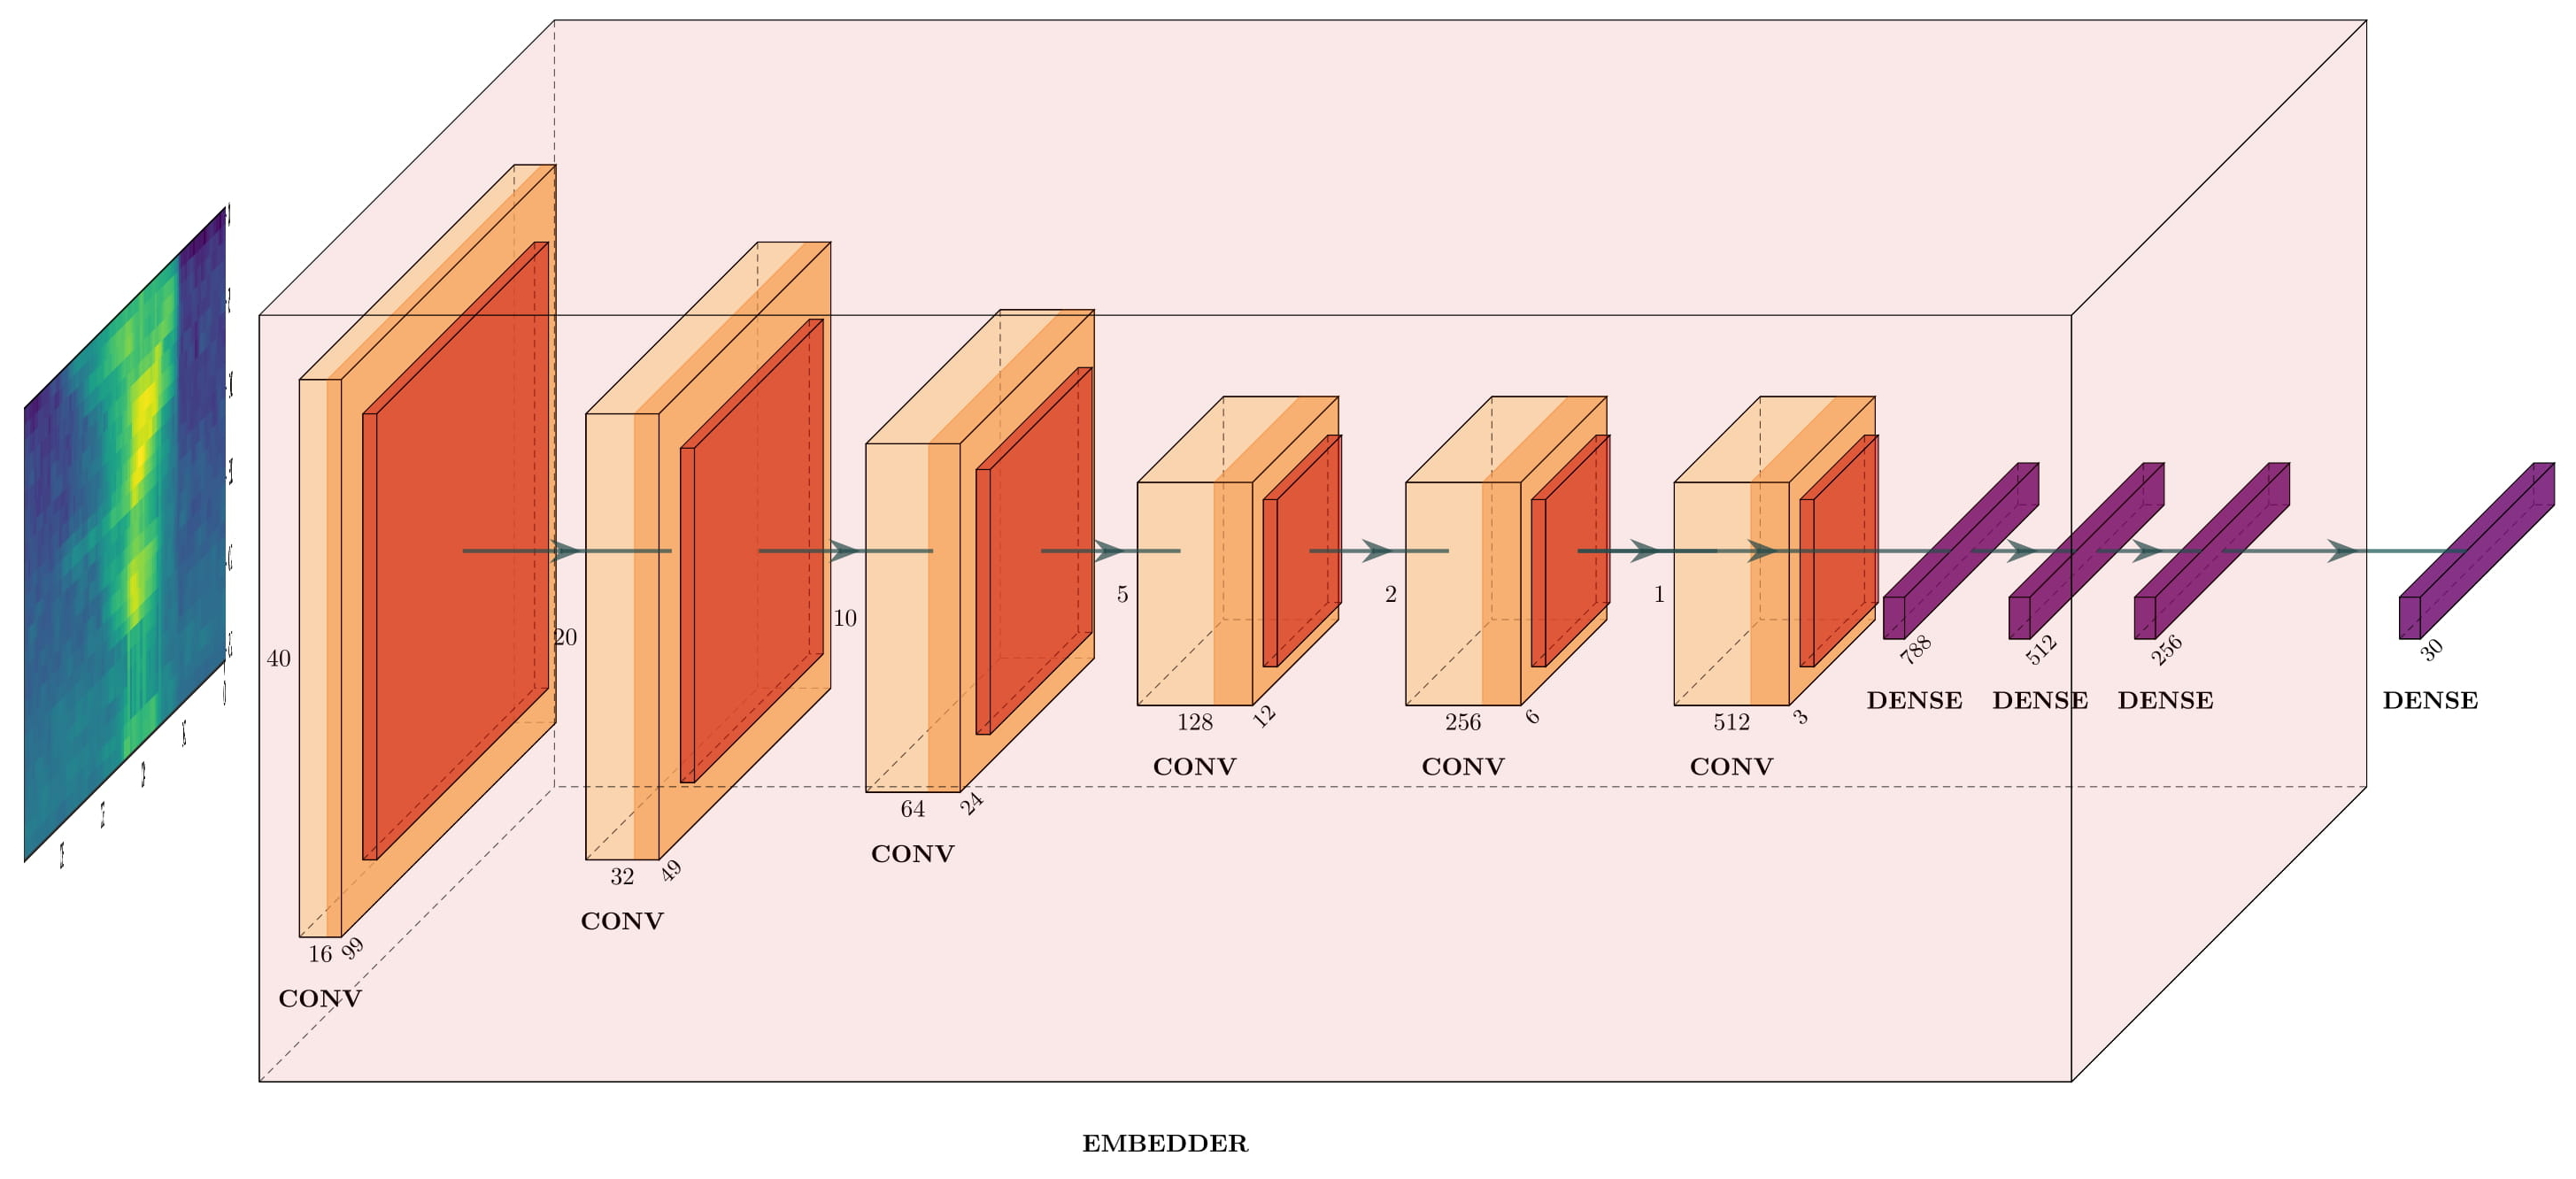
\includegraphics[width=1\linewidth, height=0.35\linewidth]{../results/kws2.jpg}
		%\caption{Feature (Embedding) Extractor}
		\label{fig:feature_embedder}
	\end{figure}
	
	\begin{itemize}
		\item<1-> We can interpret the deep network as a ``black box" that transforms the input from one representation to another.
		\item<2-> Hence, the subnetwork in the box can be considered as an \textit{embedder} that transforms the input.
	\end{itemize}
\end{frame}


\begin{frame}{KWS System}
	\begin{figure}[h]
		\centering
		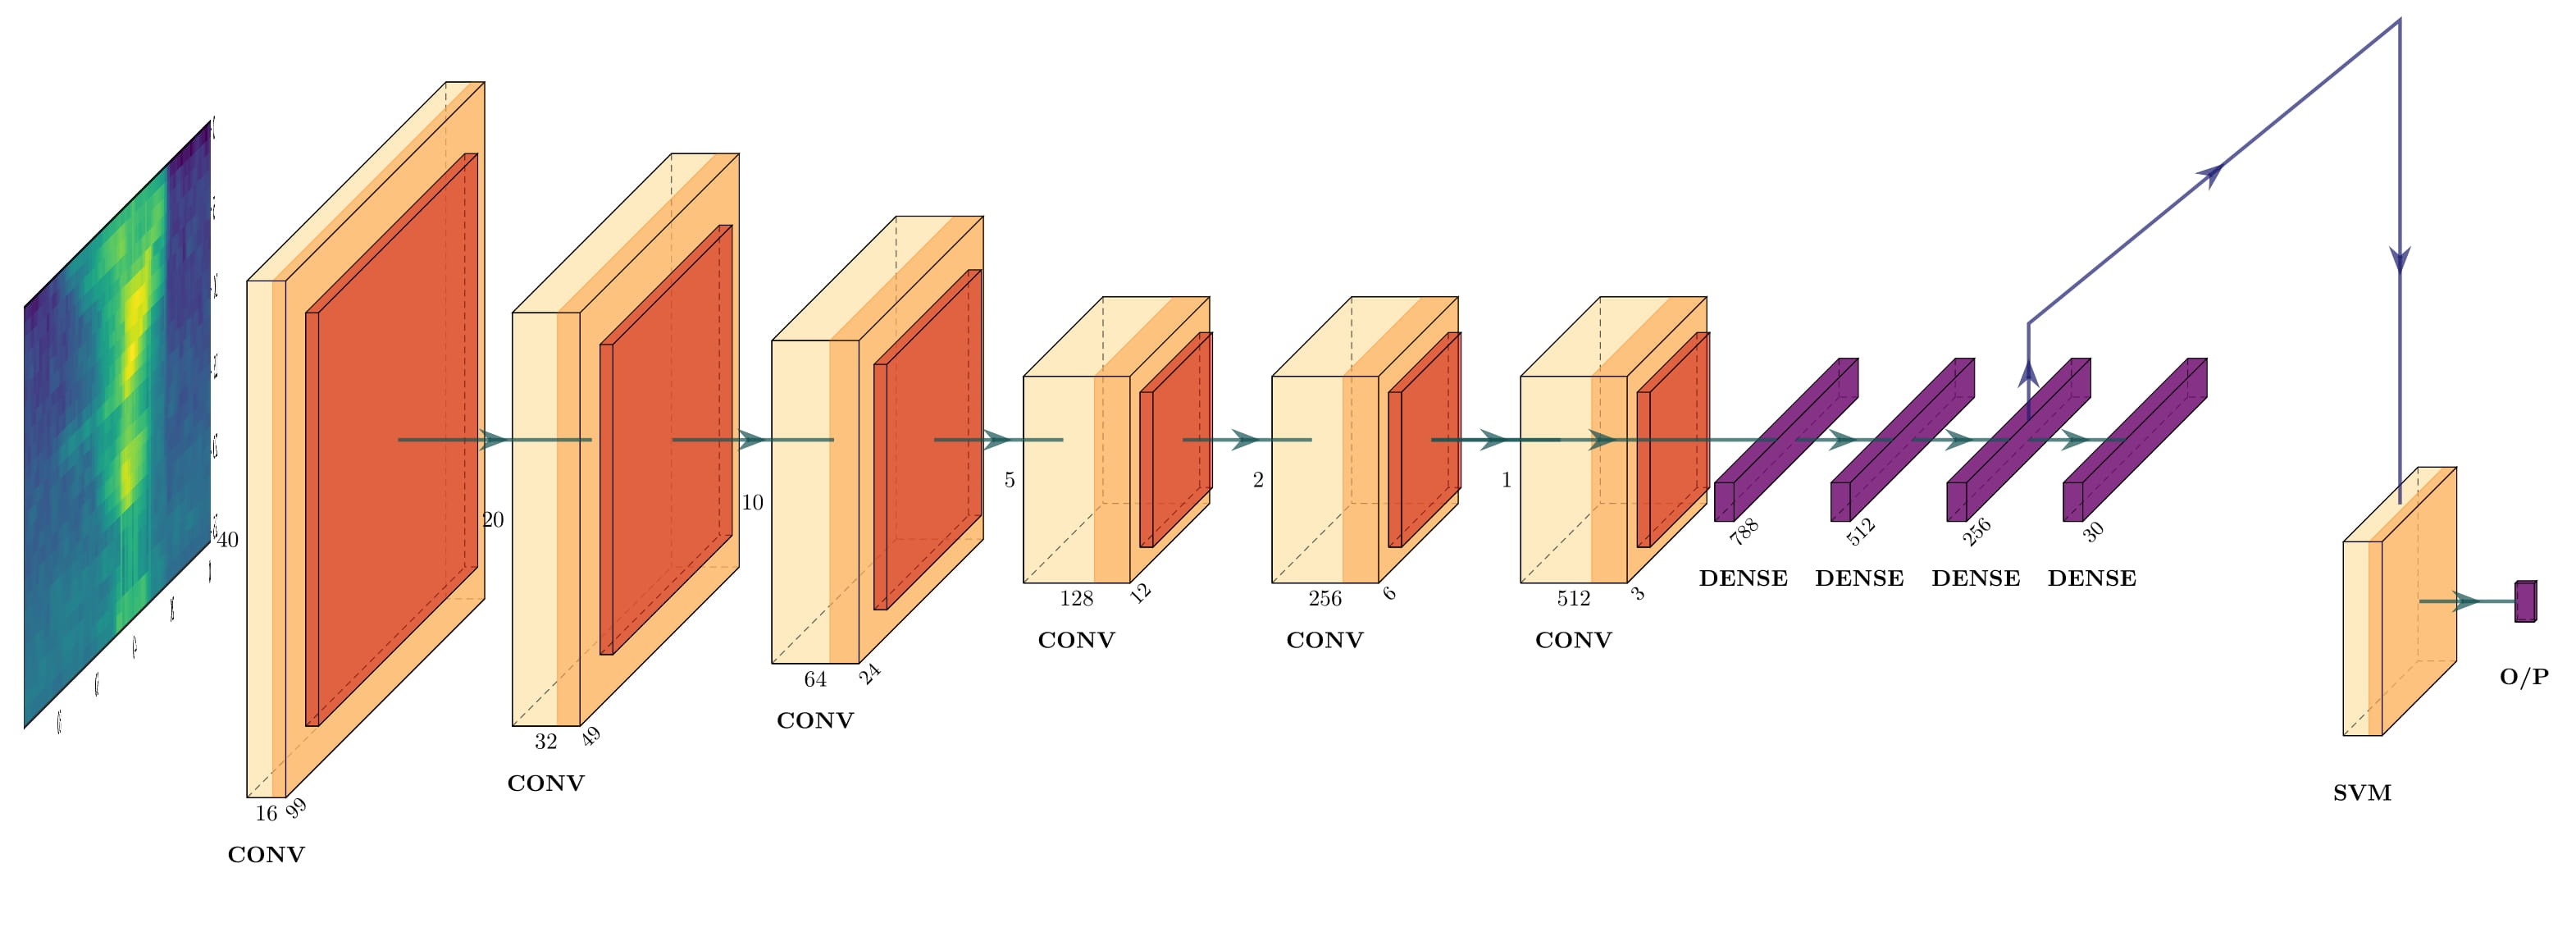
\includegraphics[width=1\linewidth, height=0.35\linewidth]{../results/kws3.jpg}
		%\caption{Feature (Embedding) Extractor}
		\label{fig:feature_embedder}
	\end{figure}

	\begin{itemize}
		\item<1-> We consider the output of the penultimate layer (256 dimension) as an \textit{embedding} of the input feature.
		\item<2-> We then train an One Class SVM (OC-SVM), used popularly for outlier detection, with these embedding as input.
	\end{itemize}
\end{frame}


\begin{frame}{One Class SVM}
	\begin{itemize}
		\item<1-> We train the OC-SVM using validation dataset of Google Speech Commands (not using the entire training dataset). We test the OC-SVM using test dataset.
		\item<2-> We select the hyperparameters of OC-SVM using tuning with \textit{scikit-optimize} library.
	\end{itemize}

	\uncover<3>{
	\begin{table}[ht]
		\begin{varwidth}[b]{0.5\linewidth}
			\centering
			\resizebox{\textwidth}{!}{
			\begin{tabular}{ l r r r }
				\toprule \hline
			    \textbf{Model size}							& \textbf{11.4MB}     \\ \hline
				Model size (Quantized) 						& $978$KB             \\ \hline
				\textbf{Real Time Factor (RTF)}	 			& \textbf{1.7ms}      \\ \hline
				Accuracy 		 							& $0.9995$            \\ \hline
				Precision			 						& $0.9942$            \\ \hline
				Recall (True Detection Rate)		 		& $0.9770$            \\ \hline
				\textbf{F1 Score}	 						& \textbf{0.9855}     \\ \hline
				\textbf{Matthews Correlation Coefficient}	& \textbf{0.9853}     \\ \hline
				False Alarm Rate (FAR)			 			& $0.0001$            \\ \hline
				\textbf{False Alarm per Hour (FA/Hr)}		& \textbf{0.0003}     \\ \hline
				True Rejection Rates (TRR)				 	& $0.9998$            \\ \hline
				False Rejection Rates (FRR)					& $0.0229$            \\ \hline
				\bottomrule
			\end{tabular}}
			\label{table:KWS}
		\end{varwidth}%
		\hfill
		\begin{minipage}[b]{0.45\linewidth}
			\centering
			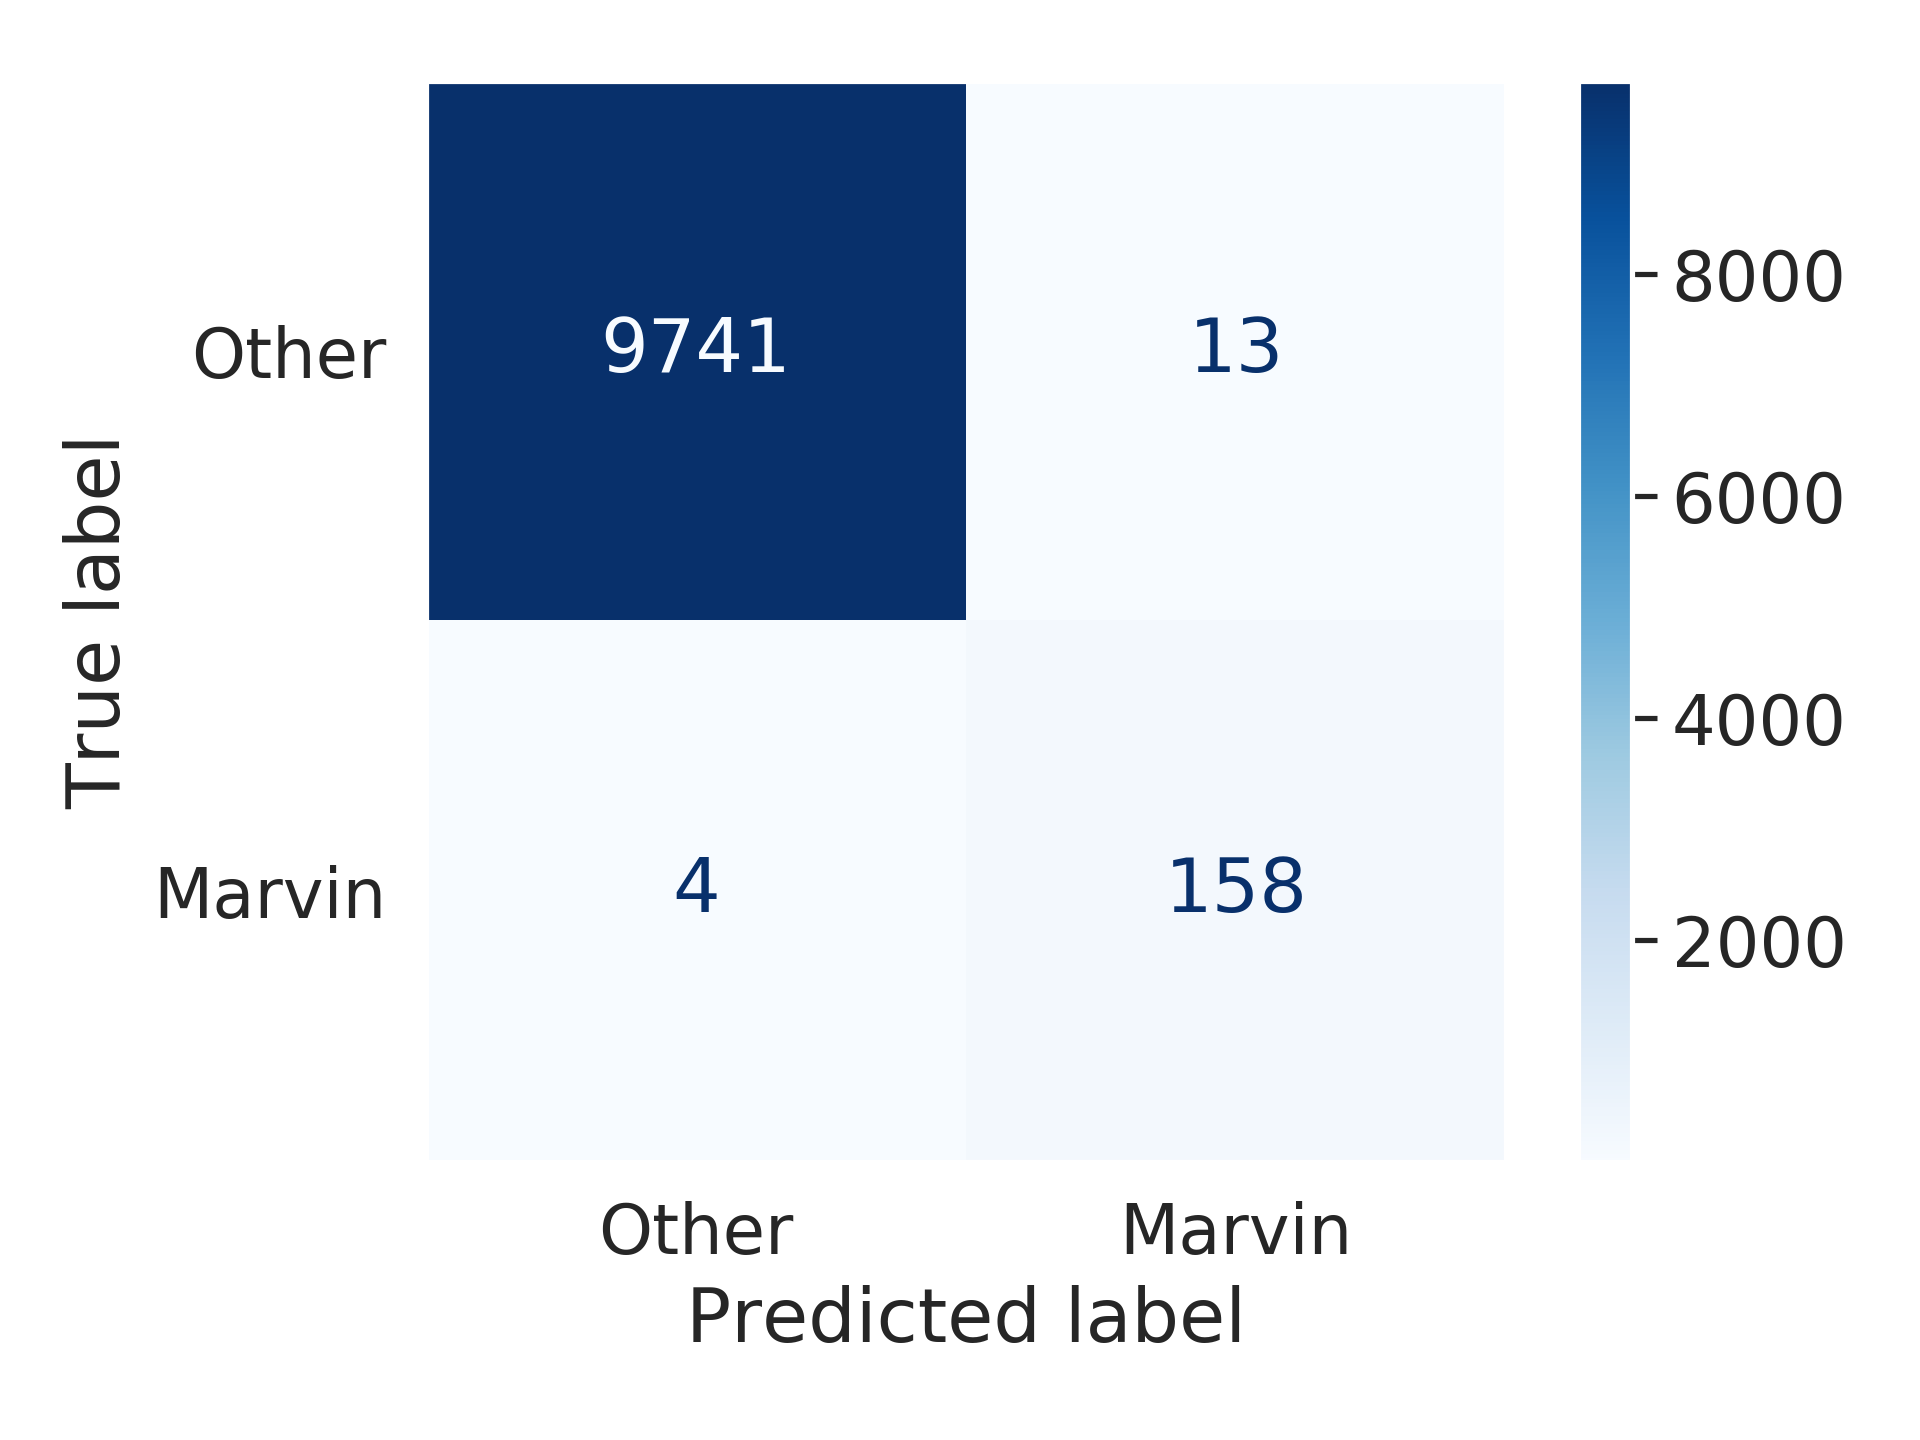
\includegraphics[width=55mm]{../results/marvin_cm_without_noise.png}
			%\captionof{figure}{2-D scatterplot of the Student Database}
			\label{fig:cm}
		\end{minipage}
	\end{table}
}
\end{frame}


\begin{frame}{Demo}
	\animategraphics[loop, autoplay,width=\linewidth]{8}{../results/demo/ezgif-frame-}{001}{150}
\end{frame}


\begin{frame}{Conclusions}
	\begin{itemize}
		\item<1-> A small footprint reconfigurable CNN-OCSVM based KWS system is proposed in this work. 
		\item<2-> The raw performance numbers shows that this model outperforms many of the models in the literature. \item<3-> However, a direct comparison is not meaningful because of the differences in the datasets and the actual keywords. 
		\item<4-> To prove this claim a lot of further work is necessary, such as performance analysis under noise and far-field conditions.
	\end{itemize}
\end{frame}


\begin{frame}
	\frametitle{Bibliography}
	\printbibliography[heading=none]
\end{frame}



\begin{frame}
	\huge{\centerline{The End}}
	
	\hspace{10em}
	
	\huge{\centerline{Questions? Suggestions?}}
\end{frame}




\end{document}
